% !TEX root =  Main.tex
\subsection{Space Software Mutation Testing Pipeline}
\label{sec:approach}

\begin{figure}[tb]
\begin{center}
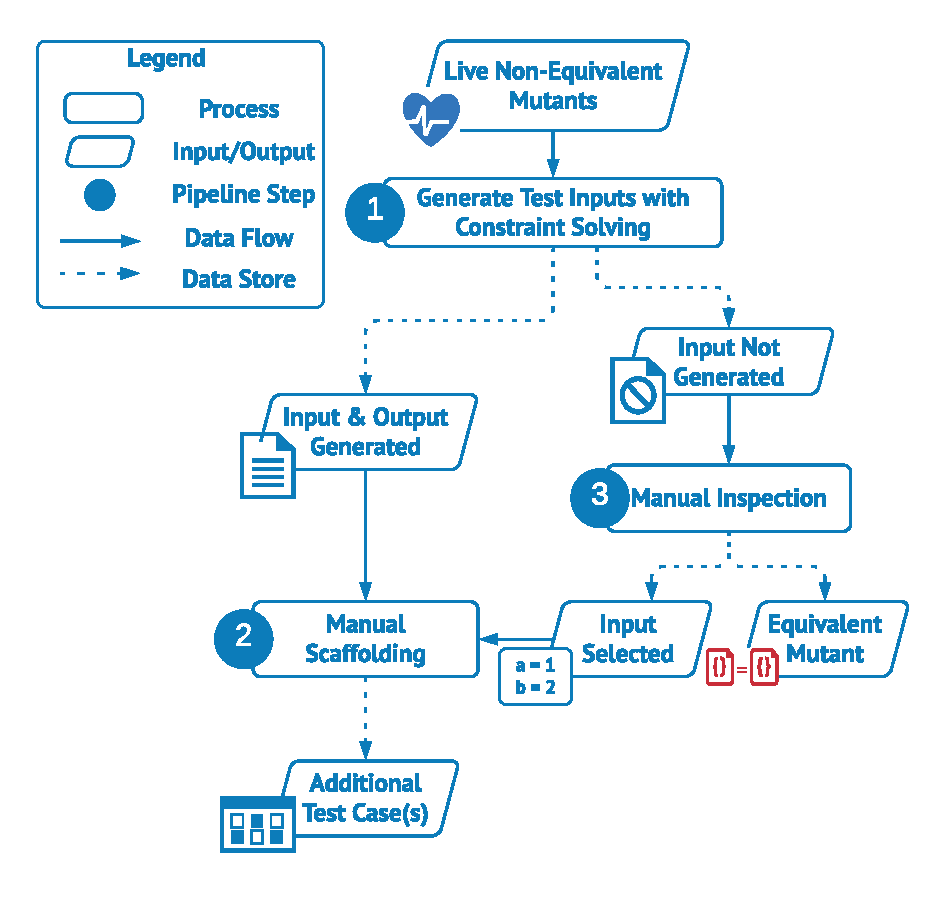
\includegraphics[width=13cm]{images/MT2}
\caption{Overview of the proposed Mutation Testing Pipeline}
\label{fig:approach}
\end{center}
\end{figure}

Figure~\ref{fig:approach} provides an overview of the mutation testing process that we propose, 
\emph{Scalable Mutation Testing for Space Software} (\APPR), based on the discussions and decisions in the previous section. We describe each step in the following paragraphs. 

\subsubsection{Step 1: Collect coverage data of the SUT test suite}

In Step 1, the test suite is executed against the software under test (SUT) and code coverage information is collected. 
More precisely, we rely on the combination of gcov~\cite{GCOV}
and GDB~\cite{GDB}, enabling the collection of coverage information for embedded systems without a file system~\cite{THANASSIS}.
% and Vector CAST~\cite{VectorCAST} 
%to record the number of times each line of code of the SUT has been exercised by a test case.

\subsubsection{Step 2: Create Mutants}

In Step 2, we automatically generate mutants for the SUT by relying on a set of selected mutation operators.
In \APPR, based on the considerations provided in Section~\ref{sec:related:operators}, we rely on an extended sufficient set of mutation operators, which are listed in Table~\ref{table:operators}.
In addition, in our experiments, we also evaluate the feasibility of relying only on the SDL operator, combined or not with OODL operators, instead of the entire sufficient set of operators.

% !TEX root =  ../Main.tex

\newcommand{\op}{\mathit{op}}
\newcommand{\ArithmeticSet}{ \texttt{+}, \texttt{-}, \texttt{*}, \texttt{/}, \texttt{\%} }
\newcommand{\LogicalSet}{ \texttt{&&}, \texttt{||} }
\newcommand{\RelationalSet}{ \texttt{>}, \texttt{>=}, \texttt{<}, \texttt{<=}, \texttt{==}, \texttt{!=} }
\newcommand{\BitWiseSet}{ \texttt{\&}, \texttt{|}, \land }
\newcommand{\ShiftSet}{ \texttt{>>}, \texttt{<<} }


\begin{table}[h]
\caption{Implemented set of mutation operators.}
\label{table:operators} 
\centering
\scriptsize
\begin{tabular}{|@{}p{4mm}@{}|@{}p{2cm}@{\hspace{1pt}}|@{}p{11.1cm}@{}|}
\hline
&\textbf{Operator} & \textbf{Description$^{*}$} \\
\hline
\multirow{7}{*}{\rotatebox{90}{\emph{Sufficient Set}}}&ABS               & $\{(v, -v)\}$	\\
\cline{2-3}
&AOR               & $\{(\op_1, op_2) \,|\, \op_1, \op_2 \in \{ \ArithmeticSet \} \land \op_1 \neq \op_2 \} $       \\
&    			  & $\{(\op_1, \op_2) \,|\, \op_1, \op_2 \in \{\texttt{+=}, \texttt{-=}, \texttt{*=}, \texttt{/=}, \texttt{\%} \texttt{=}\} \land \op_1 \neq \op_2 \} $       \\
\cline{2-3}
&ICR               & $\{i, x) \,|\, x \in \{1, -1, 0, i + 1, i - 1, -i\}\}$           \\
\cline{2-3}
&LCR               & $\{(\op_1, \op_2) \,|\, \op_1, \op_2 \in \{ \texttt{\&\&}, || \} \land \op_1 \neq \op_2 \}$            \\
&				  & $\{(\op_1, \op_2) \,|\, \op_1, \op_2 \in \{ \texttt{\&=}, \texttt{|=}, \texttt{\&=}\} \land \op_1 \neq \op_2 \}$            \\
&				  & $\{(\op_1, \op_2) \,|\, \op_1, \op_2 \in \{ \texttt{\&}, \texttt{|}, \texttt{\&\&}\} \land \op_1 \neq \op_2 \}$            \\
\cline{2-3}
&ROR               & $\{(\op_1, \op_2) \,|\, \op_1, \op_2 \in \{ \RelationalSet \}\}$            \\
&				  & $\{ (e, !(e)) \,|\, e \in \{\texttt{if(e)}, \texttt{while(e)}\} \}$ \\
\cline{2-3}
&SDL               & $\{(s, \texttt{remove}(s))\}$            \\
\cline{2-3}
&UOI               & $\{ (v, \texttt{--}v), (v, v\texttt{--}), (v, \texttt{++}v), (v, v\texttt{++}) \}$            \\   
\hline
\hline
\multirow{5}{*}{\rotatebox{90}{\emph{OODL}}}&AOD               & $\{((t_1\,op\,t_2), t_1), ((t_1\,op\,t_2), t_2) \,|\, op \in \{ \ArithmeticSet \} $       \\ 
\cline{2-3}
&LOD               & $\{((t_1\,op\,t_2), t_1), ((t_1\,op\,t_2), t_2) \,|\, op \in \{  \} \}$       \\ 
\cline{2-3}
&ROD               & $\{((t_1\,op\,t_2), t_1), ((t_1\,op\,t_2), t_2) \,|\, op \in \{ \RelationalSet \} \}$       \\ 
\cline{2-3}
&BOD               & $\{((t_1\,op\,t_2), t_1), ((t_1\,op\,t_2), t_2) \,|\, op \in \{ \BitWiseSet \} \}$       \\ 
\cline{2-3}
&SOD               & $\{((t_1\,op\,t_2), t_1), ((t_1\,op\,t_2), t_2) \,|\, op \in \{ \ShiftSet \} \}$       \\ 
%\hline
%COR               & $\{(\op_1, \op_2) \,|\, \op_1, \op_2 \in \{ \texttt{\&\&}, \texttt{||}, \land \} \land \op_1 \neq \op_2 \}$            \\
\hline
\hline
\multirow{3}{*}{\rotatebox{90}{\emph{Other}}}&LVR			& $\{(l_1, l_2) \,|\, (l_1, l_2) \in \{(0,-1), (l_1,-l_1), (l_1, 0), (\mathit{true}, \mathit{false}), (\mathit{false}, \mathit{true})\}\}$\\
&&\\
&&\\
\hline
\end{tabular}

$^{*}$Each pair in parenthesis shows how a program element is modified by the mutation operator. Th eleft element of the pair is replaced with the right element. We follow standard syntax~\cite{kintis2018effective}. Program elements are literals ($l$), integer literals ($i$), boolean expressions ($e$), operators ($\op$), statements ($s$), variables ($v$), and terms ( $t_i$, which might be either variables or literals).
\end{table}

To automatically generate mutants, we have extended SRCIRor~\cite{hariri2018srciror} to include all the 
operators in Table~\ref{table:operators}.
After mutating the original source file, our extension saves the mutated source file and keeps track of the mutation applied. 

\subsubsection{Step 3: Compile mutants}
\label{sec:appr:compile}

In Step 3, we compile mutants by relying on the build system of the SUT. To this end, we have developed a toolset that, for each mutated source file: (1) backs-up the original source file, (2) renames the mutated source file as the original source file, (3) runs the build system (e.g., executes the command \texttt{make}), (4) copies the generated executable mutant in a dedicated folder, (5) restores the original source file. 

Build systems create one object file for each source file to be compiled and then link these object files together into the final executable. 
 {In subsequent builds, they recompile only the modified files and link them to the rest.}
For this reason, since we modify at most two source files for each mutant (i.e., the mutated file and the file restored to eliminate the previous mutation), we can reuse almost all the compiled object files in subsequent compilation runs, thus speeding up the compilation of multiple mutants. The experiments conducted with our case study systems (Section~\ref{sec:evaluation}) have shown that 
%additional optimizations are not necessary to make the compilation of mutants feasible.
 {our optimization is sufficient to make the compilation of mutants feasible for large projects. Other state-of-the-art solutions introduce additional complexity (e.g., change the structure of the software under test~\cite{untch1993mutation}) that does not appear to be justified by scalability needs.}
 
 
 \REVNOV{C-P-24}{Mutants that lead to compilation errors are discarded. Concerning compilation warnings, we assume the build system of the SUT has been properly configured; more precisely, if the system should compile without warnings, the compiler is expected to be configured to treat warnings as errors otherwise mutants that lead to warning are retained.}

\subsubsection{Step 4: Remove equivalent and redundant mutants based on compiled code}

In Step 4, we rely on trivial compiler optimizations to identify and remove equivalent and redundant mutants. 
\REVNOV{C-P-15}{We compile the original software and every mutant multiple times once for each every available optimization option (i.e., \texttt{-O0}, \texttt{-O1}, \texttt{-O2}, \texttt{-O3}, \texttt{-Os}, \texttt{-Ofast} in GCC) or a subset of them.
After each execution of the compiler, we compute the SHA-512 hash summary of the generated executable.} Finally, we compare all the generated hash summaries. Hash comparison enables us to (1) determine the presence of equivalent mutants (i.e., mutants having the same hash as any of the executables generated for the original program), and (2) identify duplicate mutants (i.e., mutants with the same hash). %Mutants that are identified as being either equivalent and redundant mutants are ignored in the following steps of \APPR. 
Equivalent and redundant mutants are discarded.
The outcome of Step 4 is a set of \emph{unique mutants}, i.e., mutants with compiled code that differs from the original software and any other mutant.

Should the SUT not be compiled with compiler optimizations enabled, we identify equivalent and redundant mutants by re-executing Step 3 with compiler optimizations enabled and then apply Step 4.
%The executables generated by this additional run of Step 3 are used only to identify equivalent mutants, not to evaluate the SUT test suite, which is based on executables compiled without optimizations (otherwise test cases may fail).

\subsubsection{Step 5: Sample Mutants}
\label{sec:codeDriven:samplingStep}
\STARTCHANGEDNOV

In Step 5, we sample the mutants to be executed to compute the mutation score. 
Our pipeline supports different sampling strategies: \emph{proportional uniform sampling}, \emph{proportional method-based sampling},  \emph{uniform fixed-size sampling}, and \emph{uniform FSCI sampling}. 

The strategies \emph{proportional uniform sampling} and \emph{proportional method-based sampling} are based on the results of Zhang et al.~\cite{zhang2013operator}, who compared eight strategies for sampling mutants. 
The former is the best performing strategy in \cite{zhang2013operator} and consists of sampling mutants evenly across all functions of the SUT, i.e., sampling $r\%$ mutants from each set of mutants generated inside a same function.
 {The latter consists of randomly selecting $r\%$ mutants from the complete mutants set. This is included in our study because it is simpler to implement and proved to be equivalent to stratified sampling strategies, based on recent work~\cite{gopinath2015hard}.}

 {The \emph{uniform fixed-size sampling} strategy stems from the work of Gopinath et al.~\cite{gopinath2015hard} and consists of selecting a fixed number $N_M$ of mutants for the computation of the mutation score. Based on Gopinath et al. work, 1000 mutants guarantee an accurate estimation of the mutation score. In our empirical evaluation, we assess the accuracy obtained for $N_M$ values across the range [100;1000].}

 {In this paper, we introduce the \emph{uniform FSCI sampling} strategy that determines the sample size dynamically, while exercising mutants, based on a fixed-width sequential confidence interval approach.
With the \emph{uniform FSCI sampling} we introduce a cycle between Step 6 and Step 5 of the approach, such that a new mutant is sampled only if deemed necessary by FSCI analysis.
% of the mutation testing results collected so far. 
 More precisely, \APPR iteratively selects a random mutant from the whole set of unique mutants and exercises it using the SUT test suite. 
% The result of each mutant execution (i.e., killed or live) is treated as a Bernoulli trial that is used to compute the confidence interval according to the FSCI method. 
Based on related work, we assume that the mutation score computed with a sample of mutants follows a binomial distribution (see Section~\ref{sec:scalability}).
For this reason, to compute the confidence interval for the FSCI analysis, we rely on the Clopper-Pearson method because it provides the best results (see Section~\ref{sec:scalability}).
Mutation testing (i.e., sampling and testing a mutant) stops when the confidence interval is below a given threshold $T_{\mathit{CI}}$ (we use $T_{\mathit{CI}}=0.10$ in our experiments). More formally, given a confidence interval 
$[\mathit{L}_{S};\mathit{U}_{S}]$, with $\mathit{L}_{S}$ and $\mathit{U}_{S}$ indicating the lower and upper bound of the interval, mutation testing stops when the following condition holds:}
\begin{equation}
(\mathit{U}_{S}-\mathit{L}_{S})<T_{\mathit{CI}}.
\end{equation}

 {Unfortunately, the assumption on the estimated mutation score following a binomial distribution may not hold when a subset of the test suite is executed for every mutant (i.e., what could happen in Step 6). Without going into the details behind the implementation of Step 6, which are described in Section~\ref{sec:step:prioritize}, 
it is reasonable to expect that a reduced test suite may not be able to kill all the mutants killed by the whole test suite, i.e., the estimated mutation score may be affected by negative bias. Consequently, over multiple runs, the mean of the estimated mutation score may not be close to the \emph{actual mutation score} (i.e., the mutation score computed with the whole test suite exercising all the mutants for the SUT)
 but may converge to a lower value. 
To compute a correct confidence interval that includes the actual mutation score of the SUT, we thus need to take into account this negative bias.}

 {To study the effect of negative bias on the confidence interval, we address first the relation between the actual mutation score and the mutation score computed with the reduced test suite when the whole set of mutants for the SUT is executed. 
A mutant killed by the whole test suite has a probability $P_{\mathit{KErr}}$ of not being killed by the reduced test suite.
The probability $P_{\mathit{KErr}}$  can be estimated as the proportion of mutants (erroneously) not killed by the reduced test suite 
\begin{equation}
P_{\mathit{KErr}} = \frac{|E_R|}{|M|}
\end{equation}
with 
$E_R$ being the subset of mutants that are killed by the whole test suite but not by the reduced test suite, and $M$ being the full set of mutants for the SUT.}

The mutation score for the reduced test suite (i.e., $\mathit{MS}_R$) can be computed as

\begin{equation}
\mathit{MS}_R=\frac{K-E_R}{|M|}=\frac{K}{|M|}-\frac{E_R}{|M|}=\mathit{MS}-\frac{|E_R|}{|M|}=\mathit{MS}-P_{\mathit{KErr}}
\end{equation}

where $K$ is the set of mutants killed by the whole test suite, $M$ is the set of all the mutants of the SUT,  and $\mathit{MS}$ is the actual mutation score. Consequently, the actual mutation score can be computed as 
\begin{equation}
\label{eq:MS}
\mathit{MS}=\mathit{MS}_R+P_{\mathit{Err}_R}
\end{equation}

 {We now discuss the effect of a reduced test suite on the confidence interval for a mutation score estimated with mutants sampling. When mutants are sampled and tested with the whole test suite, the actual mutation score is expected to lie in the confidence interval $[\mathit{L}_{S};\mathit{U}_{S}]$. 
However, in the presence of a reduced test suite, we have to take into account the probability of an error in the computation of the mutation score $\mathit{MS}_R$;  $\mathit{MS}_R$ may be lower than $\mathit{MS}$ and, based on Equation~\ref{eq:MS}, we may expect the actual mutation score to lie in the interval}

\begin{equation}
\label{eq:CI}
\mathit{CI}=[\mathit{L}_{S};\mathit{U}_{S}+P_{\mathit{KErr}}]
\end{equation}

 {We can only estimate  $P_{\mathit{KErr}}$ since computing it would require the execution of all the mutants with the complete test suite, thus undermining our objective of reducing test executions. 
To do so, we can randomly select a set $M_S$ of mutants, on which to execute the whole test suite and identify the mutants killed by the reduced test suite. %\footnote{In our implementation, we record the outcome of each test case of the whole suite and then simulate the execution of the reduced test suite, thus saving time.} 
The size of the set $M_S$ should be lower than the number of mutants expected to be returned by FSCI sampling (e.g., we use $M_S'=100$ in our experiments\footnote{Though it would be possible to also estimate $P_{\mathit{KErr}}$ with FSCI, we leave it for future work}), otherwise sampling would not provide any cost reduction benefit.
Since for every mutant in $M_S$ we can determine if it is erroneously reported as not killed by the reduced test suite,
we can 
%end up with a vector of boolean evaluations $E=e_1, ..., e_n$ where each evaluation $e_i$ is equal to \emph{true} if the $i^{th}$ mutant has been erroneously indicated as not killed by the reduced test suite.
%This population of evaluations enable us to 
estimate the probability $P_{\mathit{KErr}}$ as the percentage of such mutants.
As for the case of the mutation score, these mutants tend to be positively  correlated\footnote{If a line of code contains a mutant that is not killed by the reduced test suite, it may contain another such mutant.} and, for this reason, the binomial distribution should provide a conservative estimate of the variance for $P_{\mathit{KErr}}$.} 

 {We can estimate the confidence interval for $P_{\mathit{KErr}}$ using one of the methods for binomial distributions.
We rely on the Wilson score method because it is known to perform well with small samples. 
The value of $P_{\mathit{KErr}}$ will thus lie within $[\mathit{L}_{E};\mathit{U}_{E}]$,  with $\mathit{L}_{E}$ and $\mathit{U}_{E}$ indicating the lower and upper bound of the interval.}

 {Based on Equation~\ref{eq:CI}, to ensure that the actual mutation score lies in the computed confidence interval, we should assume the worst case, i.e., $P_{\mathit{KErr}}=\mathit{U}_{E}$.
The confidence interval to be used with FSCI sampling in the presence of a reduced test suite should thus be }
\begin{equation}
\label{eq:CI:FSCI}
\mathit{CI}=[\mathit{L}_{S};\mathit{U}_{S}+\mathit{U}_{E}]
\end{equation}

 {From a more practical perspective, the effect of the term $+\mathit{U}_{E}$ is to augment the size of the interval returned by the Clopper-Pearson method; consequently, mutation sampling with a reduced test suite may lead to the execution of a larger set of mutants.}

 {When $\mathit{U}_{E}>T_{\mathit{CI}}$, the reduced test suite cannot lead to accurate results. In such cases, the test suite can be prioritized but not reduced and the confidence interval should thus be computed using the traditional Clopper-Pearson method, i.e., $[\mathit{L}_{S};\mathit{U}_{S}]$.}

 {In Section~\ref{sec:evaluation} we discuss the difference in accuracy for the different strategies.}

\ENDCHANGEDNOV

\subsubsection{Step 6: Execute prioritized subset of test cases}
\label{sec:step:prioritize}

In Step 6, we execute a prioritized subset of test cases. 
We select only the test cases that satisfy 
the reachability condition (i.e., cover the mutated statement) and  execute them in sequence.
Similarly to the approach of Zhang et al. \cite{zhang2013faster}, we define the order of execution of test cases based on their estimated likelihood of killing a mutant.
 {However, in our work, this likelihood is estimated differently than in the case of Zhang et al. because of the inapplicability of the measurements they propose in the context of system-level testing and complex systems. 
(see Section~\ref{sec:scalability}).}
%However, we redefined the criteria for the prioritization and selection of test cases because of the inapplicability of the ones proposed by Zhang et al. (see Section~\ref{sec:scalability}).

%However, we notice that such optimization may not be sufficient when test suites are particularly large; indeed, prioritizing test cases may not be sufficient to reduce execution time. For example, live mutants may lead to the execution of a large number of test cases when almost all the test cases of the test suite exercise the mutated statement. 
\REVNOV{C-P-46}{We execute only covered statements assuming that the test suite is optimal with respect to code coverage. More precisely, we addume that if a statement is not covered there is a good reason for it (e.g., it depends on hardware). 
If a statement is not covered by the test suite, there is no chance that a mutant generated in the non-covered statement can be possibly detected by any test case. 
If the test suite does not reach the required coverage there is no reason to perform mutation testing, because is already known that the test suite is not good.}

To reduce the number of test cases to be executed with a mutant, 
we should first execute the ones that more likely satisfy the necessity condition. 
This might be achieved by executing a test case that exercises the mutated statement with variable values not observed before. 
Unfortunately, in our context, the size of the SUT and its real-time constraints prevent us from recording all the variable values processed during testing. 

To determine if two test case executions exercise the mutated statement with diverse variable values, we therefore rely on code coverage.
% as a surrogate indicator of  variable values diversity.
%diversity in values assigned to the variables used in a statement. 
Indeed, a difference in the set of instructions being covered by two or more test cases that exercise a same statement may depend on the values used in such statement. For example, the definition of a variable may lead to the execution of different branches when different values are assigned across distinct executions.
However, two test case executions may also present coverage differences 
because of a diverse set of variable values used by statements other than the mutated one. 
For this reason, we restrict the scope of code coverage analysis 
to the functions belonging to a same component (i.e., a same source file).
Indeed, such functions typically present several control- and data-flow dependencies, thus 
augmenting the likelihood that a coverage difference is due to the execution of the mutated statement with a diverse set of values.

%to the mutated function, its callers, and its callees.
%to maximize the chances that a change in the behaviour of the software depends on the values used in a mutated statement, we determine that two executions likely exercise a mutated statement with diverse values by focussing on the coverage of 
%the mutated function, its callers, and its callees.
%A reduced scope is effective in determining behavioural differences based on the analysis of variable valuations~\cite{Pastore:VART:2014}.

%Since related work focuses on either statement coverage or the frequency of execution of a statement, 
Based on related work, we have identified two possible strategies to characterize test case executions based on code coverage:
\begin{itemize}
\item[S1] Compare the sets of source code statements being covered by the test cases~\cite{grun2009impact}.
%\item[C2] Identify the set of unique pairs $\langle\mathit{statement},\mathit{arity}\rangle$, where $\mathit{statement}$ is a unique identifier for the source code statement, and $\mathit{arity}$ is a symbol (i.e., $1$ or $*$) indicating if the statement has been covered one or more times.
\item[S2] Compare the number of times each statement has been covered by distinct test cases~\cite{schuler2013covering}.
\end{itemize}


To determine how dissimilar two test cases are and, consequently, how likely they exercise the mutated statement with different values, we rely on widely adopted distance metrics. 
In the case of S1, we rely on the Jaccard and Ochiai index, which are two similarity indices for binary data and have successfully been used to compare program executions based on code coverage~\cite{Zou:Ochiai:2019,Keller:Jaccard:2017,Briand:2019}. 
\REVNOV{C-P-18}{The Jaccard index is also known as \emph{intersection over union} 
it measures similarity between sets, and is defined as the size of the intersection divided by the size of the union.
The Jaccard distance measures dissimilarity between sample sets and results from subtracting the Jaccard coefficient from 1.
The Ochiai index calculates cosine similarity with binary data, it is used in molecular biology and software engineering.}
Given two test cases $T_A$ and $T_B$, the Jaccard  ($D_J$) and the Ochiai ($D_O$) distances are computed as follows:

$D_J(T_a,T_b)=1-\frac{|C_a \cap C_b|}{|C_a \cup C_b|}$ \hspace{2mm} $D_O(T_a,T_b)=1-\frac{|C_a \cap C_b|}{\sqrt{|C_a| * |C_b|}}$, 
where $C_a$ and $C_b$ are the set of coverage items exercised by the test cases $T_a$ and $T_b$, respectively.

In the case of S2, we compute the distance between two test cases by relying on the euclidean distance ($D_E$) and the cosine similarity distance ($D_C$), two popular distance metrics used in machine learning. 
\REVNOV{C-P-18}{Euclidean distance is the straight-line distance between two points in Euclidean space; precisely, the Euclidean distance between two points is the length of the line segment connecting them. In our context, the two vectors consist of the number of times teh program statements had been exercised by a test. Cosine similarity measures similarity between two vectors of an inner product space. It results from the inner product of the same vectors normalized to both have length 1, which matches the the cosine of the angle between them. It is widely adopted to measure cohesion within clusters in data mining.}
Given two vectors $V_A$ and $V_B$, whose elements capture the number of times a statement has been covered by test cases $T_A$ and $T_B$, the distances $D_E$ and $D_C$ can be computed as follows:

$D_E=\sqrt{\sum_{i=1}^{n}(A_i-B_i)^2}$ 
$D_C= \frac{\sum_{i=1}^{n}A_i*B_i}{\sqrt{\sum_{i=1}^{n}{A_i}^2}*\sqrt{\sum_{i=1}^{n}{B_i}^2}}$,
%Their main difference is that cosine similarity is used when the magnitude of the vectors should not matter.
where $A_i$ and $B_i$ refer to the number of times the i-th statement had been covered by test cases $T_A$ and $T_B$, respectively.

Figure~\ref{alg:prioritize} shows the pseudocode of our algorithm for selecting and prioritizing test cases. It generates as output
a prioritized test suite (\emph{PTS}).
Based on the findings of Zhang et al. \cite{zhang2013faster}, we first select the test case that exercises the mutated statement the highest number of times (Line~\ref{alg:prioritize:first})  { and add it to the prioritized test suite (Line~\ref{alg:prioritize:add}).}
Then, the next selected test case is the one with the largest distance from the closest test case belonging to the set of test cases already selected (Lines~\ref{alg:prioritize:selectStart} to~\ref{alg:prioritize:selectEnd}). 
%is most different than any other test case already included in the prioritized test suite.

%Then, since we aim to maximize test cases diversity, the next selected test case should be the one that is most different than any other test case already included in the prioritized test suite.
%For this reason, for each test case $n$ not selected yet (Line~\ref{alg:prioritize:notSel}), we identify the test case $t$ showing the most similar coverage (i.e., the one with the minimal distance $d$, Line~\ref{alg:prioritize:minD}). We then select the test case $n$ with the highest distance from its closest test case (Lines~\ref{alg:prioritize:selectStart} to~\ref{alg:prioritize:selectEnd}). 

The algorithm iterates as long as it identifies a test case that exercises 
the program instructions differently than the test cases already selected (Line~\ref{alg:prioritize:until}).

Test cases are then executed in the selected order. During  execution, we collect code coverage information and identify killed and live mutants.

% !TEX root =  ../Main.tex

\newcommand{\INDA}{10}
\newcommand{\INDB}{15}
\newcommand{\INDC}{5}

%\vspace{-3mm}
\begin{figure}[tb]

\begin{algorithmic}[1]

%\footnotesize
\scriptsize
\Require \emph{TS}, the test suite of the software under test
\Require \emph{Cov}, coverage information, for each test case
\Require \emph{ms}, the mutated statement
\Ensure \emph{PTS}, a list of test cases to be executed, sorted by priority
% (source inputs, follow-up inputs, output data).

\State $\mathit{TS}_m \gets$ subset of $\mathit{TS}$ that cover the mutated statement $\mathit{ms}$, based on \emph{Cov} \label{alg:prioritize:select}
\State $\mathit{PTS} \gets \mathit{new} \mathit{list}$ \textcolor{darkgray}{//this list is initially empty}
\State $\mathit{PTS} \gets$ based on \emph{Cov} select from $\mathit{TS_m}$ the test case $t$ that exercises $\mathit{ms}$ more times \label{alg:prioritize:first}
\State $\mathit{PTS} \gets \mathit{PTS} \cup t$ \textcolor{darkgray}{//include first the test case selected above}  \label{alg:prioritize:add}

\State \textbf{repeat} \label{alg:prioritize:repeat}
\State \hspace{\INDC mm} \textbf{for each} $n$ in the set ($\mathit{TS}_m$ - $\mathit{PTS}$) \textcolor{darkgray}{, which is the set of test cases not already added to $\mathit{PTS}$} \label{alg:prioritize:notSel}
\State \hspace{\INDA mm} \textbf{for each} $t$ in $\mathit{PTS}$
\State \hspace{\INDB mm} compute the distance between $t$ and $n$
\State \hspace{\INDA mm} identify $t_n$ i.e., the test case $t$ with the minimal $d$ \label{alg:prioritize:minD}
\State \hspace{\INDC mm} among all the $t_n$ identified, select the one with the highest distance $d$ \label{alg:prioritize:selectStart}
\State \hspace{\INDC mm} \textbf{if} $d > 0$ \textcolor{darkgray}{//there is at least a test case with a different coverage}
\State \hspace{\INDA mm} \textcolor{darkgray}{//note: $n$ is the test case in the set ($\mathit{TS}_m$ - $\mathit{PTS}$) closer to $t_n$}
\State \hspace{\INDA mm} $\mathit{PTS} \gets \mathit{PTS} \cup n$ \label{alg:prioritize:selectEnd}
\State \textbf{until} $d > 0$ \label{alg:prioritize:until}


\end{algorithmic}
\vspace{-3mm}
\caption{Algorithm for prioritizing test cases}
%\vspace{-0.2cm}
\label{alg:prioritize}
\end{figure}




\subsubsection{Step 7: Identify likely equivalent/redundant mutants based on coverage data}
\label{sec:algostepSeven}


In Step 7, we identify likely equivalent and likely redundant mutants by relying on code coverage information  {collected in the previous step}.

Different from related work~\cite{schuler2013covering}, since the size of a program may determine the degree of non-determinism in statement coverage, 
we identify equivalent and redundant mutants based on a threshold, instead of relying on the absolute number of methods/statements presenting differences in code coverage. 

We compute normalized distances based on the distance metrics $D_J$, $D_O$, $D_E$, and $D_C$. A mutant is considered non-equivalent when the distance from the original program is above the threshold $T_E$, for at least one test case.
Similarly, a mutant is considered non-redundant when the distance from every other mutant is above the threshold $T_R$, for at least one test case. For the identification of equivalent mutants, we consider live mutants only. To identify redundant mutants, we consider both live and killed mutants; however, killed mutants that lead to the failure of different test cases are not redundant, regardless of their distance.

\REVNOV{C-P-19}{Figure~\ref{alg:nonEquivalent:nonRedeundat} shows the algorithm for detecting non-equivalent and non-redundant mutants.
It first identify among the list of killed mutants all the non-redundant ones (Line~\ref{alg:equivalent:KNR}).
Then it identifies the non-equivalent mutants among the list of live mutants (Line~\ref{alg:equivalent:LNE}).
Finally, it further filters the list of non-equivalent mutants to keep only the ones that appear to be non-redundant (Line~\ref{alg:equivalent:LNENR}).}

% !TEX root =  ../Main.tex

\renewcommand{\INDA}{5}
\renewcommand{\INDB}{10}
\renewcommand{\INDC}{15}
\newcommand{\INDD}{20}
\newcommand{\INDE}{25}

\renewcommand{\Comment}[1]{\textcolor{darkgray}{\textit{//#1}}}

%\vspace{-3mm}
\begin{figure}[tb]

\begin{algorithmic}[1]

%\footnotesize
\scriptsize
\Require \emph{D}, the distance function to use to identify equivalent/duplicate mutants
\Require \emph{KM}, list of killed mutants
\Require \emph{LM}, list of live mutants
\Require $\mathit{Cov}_O$, coverage information for all the test cases, for the original program
\Require $\mathit{Cov}_M$, coverage information for all the executed test cases, for every mutant
\Require \emph{TS}, list of test cases
\Require \emph{TR}, test results, for all the executions
\Ensure \emph{KNR}, a list of killed, non-duplicate  mutants
\Ensure \emph{LNENR}, a list of live, non-equivalent, non-duplicate mutants
% (source inputs, follow-up inputs, output data).

%\State $\mathit{TS}_m \gets$ subset of $\mathit{TS}$ that cover the mutated statement $\mathit{ms}$, based on \emph{Cov} \label{alg:equivalent:select}
%\State $\mathit{PTS} \gets \mathit{new} \mathit{list}$ \textcolor{darkgray}{//this list is initially empty}
%\State $\mathit{PTS} \gets$ based on \emph{Cov} select from $\mathit{TS_m}$ the test case $t$ that exercises $\mathit{ms}$ more times \label{alg:equivalent:first}
\State $\mathit{KNR} \gets \mathit{identifyNonDuplicateMutants(} \mathit{KM}, \mathit{TS}, \mathit{TR}, \mathit{Cov}_M)$ \label{alg:equivalent:KNR}
\State $\mathit{LNE} \gets \mathit{identifyNonEquivalentMutants(} \mathit{LNR}, \mathit{TS}, \mathit{Cov}_M, \mathit{Cov}_O)$ \label{alg:equivalent:LNE}
\State $\mathit{LNENR} \gets \mathit{identifyDuplicateMutants(} \mathit{LNE}, \mathit{TS}, \mathit{Cov}_M)$ \label{alg:equivalent:LNENR}


\Procedure{identifyNonDuplicateMutants}{$\mathit{M},\mathit{TS},\mathit{TR},\mathit{Cov}_M$}\Comment{$M$ is a  list of mutants, $\mathit{TS}$, $\mathit{TR}$, and $\mathit{Cov}_M$ are defined above}
\State $\mathit{NR} \gets \mathit{empty} \mathit{set}$
\State $\mathit{k1} \gets $ extract and remove first element of M
\State $\mathit{NR} \gets \mathit{NR} \cup \mathit{k1}$
\While {$\mathit{M}$ not empty}
\State $\mathit{k2} \gets $ extract and remove first element of M
\For {mutant $k1$ in $\mathit{NR}$}
\State $\mathit{duplicate}=\mathit{TRUE}$
\For {test case $t$ in $\mathit{TS}$}
\If {$t$ has different result in $k1$ and $k2$ }
\State $\mathit{duplicate}=\mathit{FALSE}$
\State \textbf{break}
\Else
\State $\mathit{cov}_{k1t} \gets $ extract coverage information for test case $t$ executed with mutant $k1$
\State $\mathit{cov}_{\mathit{k2}t} \gets $ extract coverage information for test case $t$ executed with mutant $k2$
\If {$D(\mathit{cov}_{k1t},\mathit{cov}_{\mathit{k2}t}) > T_R$ }
\State $\mathit{duplicate}=\mathit{FALSE}$
\State \textbf{break}
\EndIf
\EndIf
\EndFor
\If {$\mathit{duplicate}==\mathit{FALSE}$}
\State \textbf{break} \Comment{No need to compare with all the mutants if we know that it is not duplicate}
\EndIf
\EndFor
\If {$\mathit{duplicate}==\mathit{FALSE}$}
\State $\mathit{NR} \gets \mathit{NR} \cup \mathit{k2}$
\EndIf
\EndWhile
\State \textbf{return} $\mathit{NR}$
\EndProcedure


\Procedure{identifyNonEquivalentMutants}{$\mathit{M},\mathit{TS},\mathit{Cov}_M,\mathit{Cov}_O$}\Comment{$M$ is a  list of mutants, $\mathit{TS}$, and $\mathit{Cov}_M$, and $\mathit{Cov}_O$ are defined above}
\State $\mathit{NE} \gets \mathit{empty} \mathit{set}$
\While {$\mathit{M}$ not empty}
\State $\mathit{m} \gets $ extract and remove first element of M

\For {test case $t$ in $\mathit{TS}$}
\State $\mathit{cov}_{m} \gets $ extract coverage information for test case $t$ executed with mutant $m$
\State $\mathit{cov}_{o} \gets $ extract coverage information for test case $t$ executed with original program

\If {$D(\mathit{cov}_{m},\mathit{cov}_{o}) > T_E$ }
\State $\mathit{equivalent}=\mathit{FALSE}$
\State \textbf{break}
\EndIf

\EndFor

\If {$\mathit{equivalent}==\mathit{FALSE}$}
\State $\mathit{NE} \gets \mathit{NE} \cup \mathit{m}$
\EndIf

\EndWhile

\State \textbf{return} $\mathit{NE}$
\EndProcedure



%
%
%\State \hspace{\INDA mm} \textbf{if} $\mathit{KM}$ not empty
%\State \hspace{\INDB mm} compute the distance between $t$ and $n$
%\State \hspace{\INDA mm} identify $t_n$ i.e., the test case $t$ with the minimal $d$ \label{alg:equivalent:minD}
%\State \hspace{\INDC mm} among all the $t_n$ identified, select the one with the highest distance $d$ \label{alg:equivalent:selectStart}
%\State \hspace{\INDC mm} \textbf{if} $d > 0$ \textcolor{darkgray}{//there is at least a test case with a different coverage}
%\State \hspace{\INDA mm} \textcolor{darkgray}{//note: $n$ is the test case in the set ($\mathit{TS}_m$ - $\mathit{PTS}$) closer to $t_n$}
%\State \hspace{\INDA mm} $\mathit{PTS} \gets \mathit{PTS} \cup n$ \label{alg:equivalent:selectEnd}
%\State \textbf{until} $d > 0$ \label{alg:equivalent:until}


\end{algorithmic}
\vspace{-3mm}
\caption{Algorithm for identifying non-equivalent and non-duplicate mutants}
%\vspace{-0.2cm}
\label{alg:nonEquivalent:nonRedeundat}
\end{figure}



\subsubsection{Step 8: Compute mutation score}
\label{sec:appr:score}

The mutation score is computed as the ratio of live, non-equivalent, and non-redundant mutants (hereafter, \emph{LNENR}) over the overall number of non-equivalent, non-redundant mutants identified in Step 7:

$\mathit{mutation}\ \mathit{score} = \frac{\mathit{LNENR}}{\mathit{LNENR}+\mathit{KNR}}$,
where $\mathit{KNR}$ is the number of killed, non-redundant mutants.

%Similarly,
%
%obof at lest one test case with respect
%
%
%The code coverage difference between the mutant and the original program is represented by a \textit{threshold T\%}, a difference of code coverage over a certain T\% indicates that both versions are not equivalent.
